We now shift our attention from $\mathbb{R}^d$ to the discrete domain.
Consider an undirected graph \smash{$\mathcal{G}(\mathcal{N},\mathcal{E})$} where \smash{$\mathcal{N}\coloneqq\{v_1,...,v_N\}$} is the set of nodes and $\mathcal{E}$ is the set of edges, with $(v_i,v_j)\in \mathcal{E}$ if and only if there exists an edge between $v_i$ and $v_j$ in $\mathcal{G}$. 
\emph{Graph node kernels} \smash{$k: \mathcal{N} \times \mathcal{N} \to \mathbb{R}$} are positive definite, symmetric functions defined on pairs of nodes of $\mathcal{G}$, reflecting some notion of their `closeness' via the graph edges and weights. 
$k$ captures the structure of $\mathcal{G}$, letting practitioners repurpose popular kernelised learning algorithms to the discrete domain \citep{smola2003kernels,smola-kondor}. 
Examples include the diffusion, regularised Laplacian, cosine and random walk kernels, all of which are typically considered as functions of the graph Laplacian matrix \citep{kondor2002diffusion}.
We give a short introduction in App.~\ref{app:grf_approx}.



\pg{Graph random features} 
As in the Euclidean setting, graph kernel methods scale poorly due to the $\mathcal{O}(N^3)$ time complexity of inverting the Gram matrix $\mathbf{K}\coloneqq [k(v_i,v_j)]_{i,j=1}^N$. 
In fact, even \emph{computing} $\mathbf{K}$ often incurs a cubic cost since it involves multiplying large adjacency matrices. 
Research has been dedicated to improving efficiency by approximating $\mathbf{K}$, including \emph{graph random features} (GRFs) \citep{graph_features,reid2023universal}. 
These are sparse vectors $\{\phi_\textrm{GRF}(v_i)\}_{i=1}^N \subset \mathbb{R}^N$ that satisfy $\mathbf{K}_{ij} = \mathbb{E} \left [ \phi_\textrm{GRF}(v_i)^\top \phi_\textrm{GRF}(v_j) \right ]$, so their dot product is equal to the true graph kernel in expectation.
GRFs are constructed in subquadratic time. 

\pg{Coupled random walks}
For GRFs, the `frequencies' $\{\boldsymbol{\omega}_i\}_{i=1}^m$ are \emph{simple random walks}: sequences of graph nodes \smash{$(v_i)_{i=1}^l$} with \smash{$(v_i,v_{i+1}) \in \mathcal{E}$}. 
At every timestep, the walker chooses one of its neighbours uniformly and at random.
The length of the walk $l$ is also a random variable, drawn from a geometric distribution \smash{$l \sim \textrm{G}(p), p \in (0,1)$}. In other words, the walker terminates with probability $p$ at every timestep.
Random walks are usually taken to be independent, but this can lead to slow mixing times, poor efficiency and high kernel estimator variance \citep{alon2007non,zhou2015leveraging}. 
%Taking inspiration from successful variance-reduction techniques for Euclidean samples \citep{dick2013high,yu2016orthogonal}, 
A natural question is: \emph{can we couple graph random walks to improve the convergence of GRFs?} 

Sec.~\ref{sec:rffs_and_rlfs} couples Gaussian vector norms. 
A simple, analogous approach to couple random walks is via their \emph{lengths}. 
%\footnote{Walker \emph{directions} can also be coupled for additional variance reduction \citep{reid2023repelling}, but our work will not consider (and can be easily combined with) this complementary approach.} 
For GRFs, the constraint for unbiasedness is that the marginal distribution of each variable $l$ must remain geometric. 
\citet{reid2023quasi} proposed a simple, ad-hoc algorithm to achieve this called \emph{antithetic termination}, which directly anticorrelates the walkers' termination events at every timestep (see App.~\ref{app:antithetic_term}). 
They provide asymptotic theoretical guarantees, but only for particular choices of graph kernel. 
In the next section, we will see that our novel method of \emph{optimising} a coupling with data performs much better. 

\begin{figure}
\centering \hspace{-8mm}
    \includestandalone{grfs_master_schematic}
\caption{Schematic overview of $\sigma$-coupled GRFs with $\sigma=24351$.
\emph{Left}: permutation density with uniform marginals. 
\emph{Centre}: bipartite matching between quantiles of geometric distributions over walk lengths. 
\emph{Right}: ensemble of graph random walks with lengths to be coupled.}\label{fig:main_grfs_schematic} 
\end{figure} \vspace{-2mm}

\subsection{Approximating and solving the OT problem for GRFs} \label{sec:approximating_and_solving_grfs_ot}
Here, we present our novel approach for formulating and approximately solving the variance reduction OT problem with GRFs.
It works by mapping to a corresponding \emph{bipartite matching problem} which we can solve efficiently with linear programming techniques.
Fig.~\ref{fig:main_grfs_schematic} gives a visual overview.


\pg{Constructing GRFs from random walks} %GRFs are constructed differently to RFFs and RLFs. 
To obtain $\phi_\textrm{GRF}(v_i) \in \mathbb{R}^N$, one samples $m$ random walks \smash{$\{\boldsymbol{\omega}_k^{(i)}\}_{k=1}^m$} out of node $v_i \in \mathcal{N}$ and averages their `projections', \vspace{0mm}
\begin{equation} \label{eq:projection_func}
    \phi_\textrm{GRF}(v_i) = \frac{1}{m} \sum_{k=1}^m \psi( \boldsymbol{\omega}_k^{(i)}).
\end{equation} 
The projection function $\psi(\cdot): \Omega \to \mathbb{R}^N$ maps from the set of graph random walks \smash{$\Omega \coloneqq \left \{(v_i)_{i=1}^l \,|\, v_i \in \mathcal{N}, (v_i,v_{i+1}) \in \mathcal{E}, l \in \mathbb{N} \right \}$} to a sparse $N$-dimensional feature vector satisfying $k(v_i,v_j) = \mathbb{E}_{\boldsymbol{\omega}^{(i)}, \boldsymbol{\omega}^{(j)}}[\psi(\boldsymbol{\omega}^{(i)})^\top \psi(\boldsymbol{\omega}^{(j)})]$. 
$\psi(\cdot)$ depends on the particular kernel being approximated.
We direct the reader to the work of \citet{reid2023universal} for an introduction to GRFs, and also provide background in App.~\ref{app:grf_approx}. 
$\psi(\cdot)$ is a complicated function; it is difficult to reason about analytically but straightforward to compute for a particular walk. 
Moreover, its input walks are discrete random variables so $\psi(\cdot)$ is \emph{not} differentiable with respect to the lengths \smash{$l_k^{(i)}$} (where $k=1,...,m$ and $v_i \in \mathcal{N}$ is the walker's start node).
This precludes straightforward gradient-based optimisation (Sec.~\ref{sec:copulas}). 

\pg{A pair of walkers} Initially consider just $m=2$ walkers. 
The kernel estimator $\widehat{k}(v_i,v_j)$ is
\begin{equation}
    \widehat{k}(v_i,v_j) = \phi_\textrm{GRF}(v_i)^\top \phi_\textrm{GRF}(v_j) = \frac{1}{4} \left( \psi( \boldsymbol{\omega}_{1}^{(i)}) + \psi( \boldsymbol{\omega}_{2}^{(i)}) \right)^\top \left( \psi( \boldsymbol{\omega}_{1}^{(j)}) + \psi( \boldsymbol{\omega}_{2}^{(j)}) \right),
\end{equation}
which is unbiased provided (i) the marginal distribution of each $\boldsymbol{\omega}_{1,2}^{(i,j)}$ is a simple random walk with geometrically distributed length (hereafter denoted $\eta_\textrm{G}$) and (ii) walks from node $v_i$ are independent from walks from node $v_j$. 
The variance of the estimator depends on
\begin{equation}
    \mathbb{E}\left( \widehat{k}(v_i,v_j) ^2\right) = \frac{1}{16}  \mathbb{E}_{\boldsymbol{\omega}_{1,2}^{(i,j)}} \left(\left [\left( \psi( \boldsymbol{\omega}_{1}^{(i)}) + \psi( \boldsymbol{\omega}_{2}^{(i)}) \right)^\top \left( \psi( \boldsymbol{\omega}_{1}^{(j)}) + \psi( \boldsymbol{\omega}_{2}^{(j)}) \right) \right]^2 \right),
\end{equation}
where the expectation is taken over both the \emph{directions} and \emph{lengths} of the random walks. 
\vspace{0.5mm}Suppose the directions remain independent, but the lengths \smash{$l_1^{(i)}$} and \smash{$l_2^{(i)}$} (and likewise \smash{$l_1^{(j)}$} and \smash{$l_2^{(j)}$}) are to be coupled for variance reduction, analogously to the vector norms in Sec.~\ref{sec:rffs_and_rlfs}. 
Let $\mathbb{E}_\textrm{dirs}$ denote the expectation over the walkers' directions. 
We want to minimise:
\small
\begin{equation} \label{eq:ot_formulation}
    \mathbb{E}_{(l_1^{(i)},l_2^{(i)}) \sim \mu, (l_1^{(j)},l_2^{(j)}) \sim \mu} \mathbb{E}_\textrm{dirs} \left (  \left [ \left( \psi( \boldsymbol{\omega}_{1}^{(i)}) + \psi( \boldsymbol{\omega}_{2}^{(i)}) \right)^\top \left( \psi( \boldsymbol{\omega}_{1}^{(j)}) + \psi( \boldsymbol{\omega}_{2}^{(j)}) \right) \right]^2 \right) \textrm { for } {\mu \in \Lambda_2(\eta_\textrm{G})}.
\end{equation}
\normalsize
 %, i.e.~which neighbour they choose at each timestep.
%), conditioned on particular lengths \smash{$\{l_1^{(i)},l_2^{(i)},l_1^{(j)},l_2^{(j)} \}$}. 

\vspace{-1mm}
\pg{OT, permutation densities and bipartite matchings}
The OT problem in Eq.~\ref{eq:ot_formulation} is analytically intractable.
%; it is unclear whether the cost function it can even be written in closed form.
To make progress, we must make approximations.
We report \textbf{full details} in App.~\ref{app:what_are_the_approximations}, limiting the main text to a high-level discussion of the main points.


First, to make the objective amenable to Monte Carlo approximation, we move $\mathbb{E}_\textrm{dirs}$ inside the square. 
This is because, unlike the expression in Eq.~\ref{eq:ot_formulation}, \smash{$\mathbb{E}_\textrm{dirs} ( \psi( \boldsymbol{\omega}_{1,2}^{(i,j)}) )$} can be efficiently estimated by simulating random walks. 
Second, we must optimise amongst the class of couplings 
$\Lambda_2(\eta_\textrm{G})$, joint distributions of two discrete random variables with geometrically distributed marginals.
As in Sec.~\ref{sec:copulas}, a sensible numerical approach is to limit oneself to a tractable subclass of $\Lambda_2(\eta_\textrm{G})$. 
Taking inspiration from numerical OT, consider the family of measures \smash{$\pi^{(\sigma)}$} on $[0,1]^2$ described by the \emph{permutation densities} 
$p_\sigma(x,y) \coloneqq n 1_{\sigma(\lceil nx \rceil) = \lceil ny \rceil}$,
 with $\sigma$ a permutation of order $n$ (that is, a bijection $\sigma: [\![n]\!] \to [\![n]\!]$). 
The unit square is split into a $n\times  n$ grid where each row and column has a single `tile' of probability density $n$ and is $0$ otherwise (Fig.~\ref{fig:main_grfs_schematic} left).
Both marginal distributions of $\pi^{(\sigma)}$ are uniform on $[0,1]$ and are transformed to a probability distribution $\eta$ by pushing forward with the inverse CDF, \smash{$F_\eta^{-1}(\cdot) \coloneqq \inf \{x \in \mathbb{R}: F_\eta(x) \geq \cdot \}$}. 
Transforming both coordinates in this way yields a joint measure \smash{$\mu^{(\sigma)} \in \Lambda_2(\eta)$} which will give an unbiased estimator. 
%We refer to these as \emph{$\sigma$-couplings}, and remark that 
$n!$ such couplings exist for a given permutation order $n$; we aim to efficiently find the one with the lowest variance.

The permutations $\sigma \in S_n$ can be interpreted as \emph{matchings} between the $n$ quantiles of the geometric distributions over the lengths of a pair of walkers (Fig.~\ref{fig:main_grfs_schematic} centre).
With the correct choice of $\sigma$, they can ensure that e.g.~if one of the walk lengths is short then the other tends to be long, diversifying the ensemble (Fig.~\ref{fig:main_grfs_schematic} right).
Optimising $\sigma$, the approximate OT problem can be written
\small
\begin{equation} \label{eq:main_approx_ot_formulation_matching}
    \sigma^* = \arg \min_{\sigma \in S_n}  \sum_{q_1 \in [\![n]\!]} \sum_{q_2 \in [\![n]\!]} \left [ \left( \widehat{\psi}( q_{1}^{(i)}) + \widehat{\psi}( \sigma(q_1)^{(i)}) \right)^\top \left( \widehat{\psi}( q_{2}^{(j)}) + \widehat{\psi}( \sigma(q_2)^{(j)}) \right) \right]^2 
\end{equation}
\normalsize
where\vspace{1mm} \smash{$\widehat{\psi}(q^{(i)}) \coloneqq \mathbb{E}_{u \sim \mathcal{U}((\frac{q-1}{n}, \frac{q}{n}])} \left( \mathbb{E}_\textrm{dirs}{\psi}( F^{-1}_{\eta_\textrm{G}} (u)^{(i)})\right)$}.
$\mathcal{U}((a,b])$ is the uniform distribution on the interval $(a,b]$. % and \smash{$F^{-1}_{\eta_\textrm{G}}$} is the left-continuous inverse CDF of \smash{$\eta_\textrm{G}$}. 
Eq.~\ref{eq:main_approx_ot_formulation_matching} is a \emph{quadratic assignment problem} \citep{finke1987quadratic, burkard1998quadratic}.
This family is generally NP hard, but in our case the cost function has some convenient extra symmetric structure. 
In fact, the following is true. 
\begin{theorem}[Solving Eq.~\ref{eq:main_approx_ot_formulation_matching} exactly] \label{thm:exact_soln}
Given a set of vectors \smash{$\{\widehat{\psi}( q^{(i,j)})\}_{q=1}^n \subset \mathbb{R}^N$},  
Eq.~\ref{eq:main_approx_ot_formulation_matching} can be solved with high probability in time complexity independent of $N$. Moreover, in the special case where $i=j$, it can be solved in polynomial time in $n$ (under mild technical assumptions on the set). % provided the set is $\epsilon$-separated (see Def.~\ref{def:eps_sep}).
\end{theorem}
\emph{Proof sketch.} Details and definitions are in App.~\ref{sec:quad_grfs}. 
The time complexity can be made independent of the number of nodes $N$ by performing dimensionality reduction using the celebrated Johnson-Lindenstrauss transformation \citep{dasgupta_jlt}, which preserves pairwise dot products with high probability. 
In the special case $i=j$, Eq.~\ref{eq:main_approx_ot_formulation_matching} can be rewritten as finding a permutation $\sigma$ that minimises the $L_2$ norm of some particular $N^2$-dimensional vector.
In App.~\ref{sec:quad_grfs} we provide a novel algorithm to achieve this efficiently by projecting onto a sequence of random Gaussian vectors, requiring only a mild geometrical condition called $\epsilon$-separation. See Lemma \ref{lemma:k_matching_lemma} for full details. \qed  

More pragmatically, one can set $q_1 = q_2$ to simplify to a related \emph{linear assignment problem}, which can be solved efficiently in time $\mathcal{O}(n^3)$ using e.g.~the Hungarian algorithm \citep{kuhn1955hungarian}.
We empirically investigate how this final approximation modifies the objective in App.~\ref{app:what_are_the_approximations}.
Taking the optimal permutation and corresponding coupling \smash{$\mu^{(\sigma)}$}, we define \emph{$\sigma$-coupled GRFs} as follows.


\color{black}

\begin{tcolorbox}[colback=gray!10!white,colframe=gray!50!black,arc=0mm,boxrule=0.5pt]
\begin{definition}[$\sigma$-coupled GRFs] \label{def:coupled_grfs_def}
GRFs are \emph{$\sigma$-coupled} if they are constructed using pairs of random walks with lengths drawn from the coupling \smash{$\mu^{(\sigma)}$}, with the optimal permutation $\sigma$ obtained by solving a matching problem between the quantiles of the distributions over walk lengths (specifically, Eq.~\ref{eq:tractable_ot_formulation} in App.~\ref{app:what_are_the_approximations}).
\end{definition}
\end{tcolorbox}

%\pg{Discussion}
%Optimising the permutation $\sigma$ (and corresponding coupling $\mu^{(\sigma)}$) is the same as optimising a bipartite matching between the quantiles of the geometric distributions over the lengths of graph random walks. 
%This is effective because we can condition that, for example, if one walk is short then the other is long. 
%This means that sampled walks tend to look more `diverse' and capture different lengthscales, representing the underlying graph node kernel more accurately. 
%Even though the series of approximations required to arrive at a tractable objective mean that we are no longer exactly minimising the kernel estimator variance, this intuition is preserved when we arrive at Eq.~\ref{eq:tractable_ot_formulation}. 
Besides being easy to optimise and sample from, there are also more rigorous OT motivations for the choice of $\sigma$-couplings \smash{$\mu^{(\sigma)}$}.
They relate to the asymptotic behaviour of \smash{$\mu^{(\sigma)}$} as the permutation order $n \to \infty$ and the \emph{stability of OT plans} \citep{villani2021topics}. 
We defer this technical point to App.~\ref{app:discrete_ot_theory}. 
As in Sec.~\ref{sec:copulas}, another interesting question is whether one could couple the lengths of $m>2$ walkers.
This is challenging and has received little attention in the literature. 
One possibility would be to combine $m-1$ permutations, finding a minimum-weights $m$-partite matching with all subgraphs constrained to be complete $K_m$.
Another approach would be to approximately solve this multi-marginal OT problem using the Sinkhorn-Knopp algorithm \citep{sinkhorn1967concerning, cuturi2013sinkhorn}.
%, adding an entropy regularisation term to the objective to make it smooth and strictly convex then solving dual problem by coordinate ascent .
%We defer detailed investigation to future work.

\pg{Broader applicability} As a final remark, the utility of our algorithm extends to graph-based estimators beyond GRFs. 
For example, it can be used to improve estimates of the \emph{PageRank vector}, a popular measure of the importance of the nodes of a graph proposed by \cite{page1998pagerank} to rank websites in search engine results.
$\sigma$-couplings consistently match or beat the previous best algorithm for coupling walk lengths \citep{reid2023quasi}.
See Fig.~\ref{fig:pagerank_results} in App.~\ref{app:pagerank} for the full results.

\vspace{-3mm}\subsection{Experiments with $\sigma$-coupled GRFs} \label{sec:graph_gp_experiments} \vspace{-2mm}
We now empirically evaluate $\sigma$-coupled GRFs for variance reduction of graph node kernel estimates. 
For real-world graphs, we show that lower variance unlocks better approximate inference with scalable graph-based Gaussian processes (GPs), a novel application of GRFs. 

 \textbf{Gram matrix approximation.} GRFs take the \emph{termination probability} $p_\textrm{halt}$ as a hyperparameter, determining the rate of decay of the geometric distribution over walk length.
A smaller value of $p_\textrm{halt}$ samples longer walks and gives more accurate kernel estimates, but takes longer to run.
The optimal coupling changes depending on $p_\textrm{halt}$.
We consider the values $p_\textrm{halt} \in \{0.1,0.2,0.3,0.4,0.5\}$, finding the optimal permutation $\sigma$ in each case.
To find the optimal $\sigma$, we solve the matching problem (App.~\ref{app:what_are_the_approximations}) \begin{wrapfigure}{r}{0.45\textwidth}
\vspace{-2mm} \hspace{-4mm} \centering
    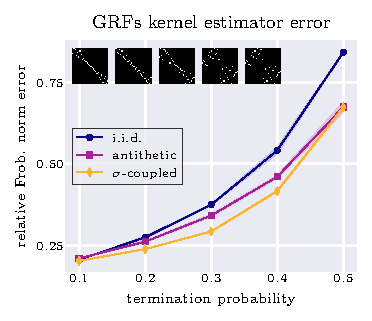
\includegraphics{images/cora_grfs.pdf} 
     \vspace{-4mm}
\caption{Kernel estimator error vs termination probability. Insets show permutations for $p_\textrm{halt}\in\{0.1,0.2,0.3,0.4,0.5\}$.}\label{fig:permuton_grf} \vspace{-4mm}
\end{wrapfigure}for a random Erd\H os-R\'enyi graph with $N=100$ nodes, taking a permutation order $n=30$ and choosing the $2$-regularised Laplacian kernel as our target. 
We use the Hungarian algorithm, averaging the cost matrix over every possible node pair $(v_i,v_j)\in \mathcal{N}^2$. % to find a coupling that reduces the variance of all entries of the Gram matrix.
Having computed couplings $\mu^{(\sigma)}$ for each value of $p_\textrm{halt}$, we then test the corresponding $\sigma$-coupled GRFs on a variety of real-world graphs. 
Fig. \ref{fig:permuton_grf} shows the results for \lstinline{cora} ($N=2708$), with the rest left to App.~\ref{app:more_grf_results}.
We plot the relative Frobenius norm error of the Gram matrix approximation \smash{$\|\mathbf{K} - \widehat{\mathbf{K}}\|_\textrm{F} / \|\mathbf{K}\|_\textrm{F}$} with walkers that are i.i.d., antithetic \citep{reid2023quasi} or $\sigma$-coupled. 
For each $p_\textrm{halt}$, $\sigma$-coupled GRFs give equally good or smaller kernel estimator errors. 
Our OT approach often substantially outperforms antithetic termination: a data-independent, hard-coded algorithm designed specifically to improve GRFs \citep{reid2023quasi}.
We include visualisations of the optimal permutations for different values of $p_\textrm{halt}$ in the inset, verifying that the $\sigma$-coupling adapts to different hyperparamaters.



\pg{Novel application: $\sigma$-coupled GRFs for scalable graph-based GPs}
We now apply $\sigma$-coupled GRFs to scalable graph-based Gaussian processes (GPs), where improved estimation of the covariance function permits better approximate inference.
Scalable GPs are a novel application of GRFs that may be of independent interest \citep{borovitskiy2021matern, mostowsky2024geometrickernels}. %; we discuss this in App.~\ref{app:grfs_for_gps}. 

%\emph{Gaussian processes} (GPs) are an indispensible workhorse of probabilistic machine learning, providing a framework for learning unknown functions in a manner that incorporates prior information and provides well-calibrated uncertainty estimates \citep{williams2006gaussian}. 
%In settings where kernels based on Euclidean distance are unsuitable, \emph{graph-based GPs} -- where the covariance function is a graph node kernel -- provide a popular alternative. 
%Like their Euclidean counterparts, graph-based GPs suffer from poor $\mathcal{O}(N^3)$ scalability as the size of graph grows on account of the need to materialise and invert a big Gram matrix. 
%In analogy to \emph{sparse spectrum Gaussian processes} in $\mathbb{R}^d$ \citep{lazaro2010sparse}, we propose to use GRFs to replace the true covariance function with a sparse, unbiased MC estimate, increasing scalability and unlocking applications on very large graphs. 
%A natural question is whether using length-coupled GRFs, which we have seen give more accurate graph node kernel estimates, will make performance even better.

Consider the task of \emph{probabilistic graph interpolation}.
This aims to predict unknown graph function values, along with principled uncertainty estimates, from an observed set \citep{pfaff2020learning}.
Take mesh graphs $\mathcal{G}$ where every node $v_i \in \mathcal{N}$ has a normal vector \smash{$\boldsymbol{n}_i \in \mathbb{R}^3$} \citep{trimesh}. 
Our task is to predict the $z$-components of a masked set, \smash{$\{(\boldsymbol{n}_i)_z\}_{i=1}^{N_\textrm{test}}$} with $N_\textrm{test}= \lfloor 0.05N \rfloor$.
To achieve this, we use a graph-based GP with a heat kernel covariance function. 
We compute a sparse, unbiased approximation of this kernel using GRFs with $\{16,32,64\}$ walkers that are i.i.d., antithetic \citep{reid2023quasi} or $\sigma$-coupled. 
%For the length-coupled walkers, the permutation is optimised on a random 
%Erd\H os-R\`enyi graph ($N=100$, $p=0.4$, $n=30$).
Details of GP hyperparameter optimisation are given in App.~\ref{app:grf_gp_details}.
Fig.~\ref{fig:graph_gps_results_2} shows the results. 
For mesh graphs of different sizes (the largest as big as $8700$ nodes), we plot the relative Frobenius norm error of the Gram matrix approximation, the test root mean square error (RMSE), and the KL divergence to the true posterior.
Our variance reduction method unlocks more accurate predictions and better uncertainty quantification, sometimes by a factor of $>2$. 
\vspace{-4mm}
\begin{figure}[H] 
    \centering \hspace{-12mm}
    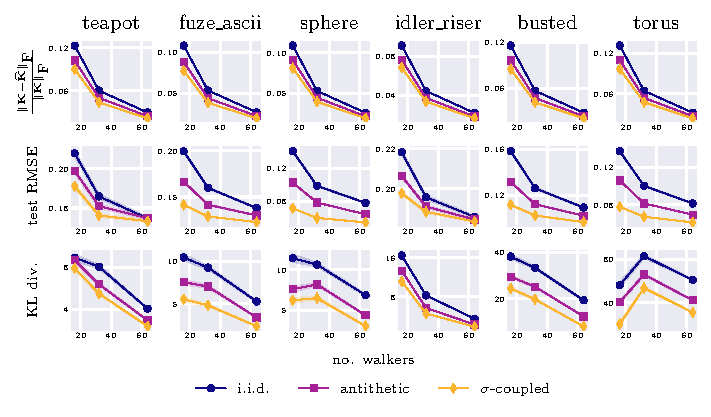
\includegraphics{images/tuned_graph_gps.pdf}
    \vspace{-3.5mm}
    \caption{Graph GP regression. Rows show the kernel estimation error, test set RMSE, and KL-divergence between the true and approximate posterior. Lower is better.
    $\sigma$-coupled GRFs give better predictions and uncertainty estimates, sometimes by a factor of $>2$. Standard errors are shaded.}
    \label{fig:graph_gps_results_2} \vspace{-5mm}
\end{figure}

\pg{Probabilistic interpolation of traffic data}
%To further demonstrate, 
We also train a scalable graph-based GP on a traffic flow dataset of the highways of San Jose, California, curated by \citet{borovitskiy2021matern} using  data from \citet{chen2001freeway} and OpenStreetMap.
The graph has $1016$ nodes, with speed only known at $325$. 
We use $250$ randomly-chosen nodes as training data and the remainder as test data.
With this sparse, noisy dataset, $\sigma$-coupled GRFs again give substantially better predictions and uncertainty estimates.
Fig.~\ref{fig:traffic} in App.~\ref{sec:traffic_expt} shows the full results.















